\documentclass[12pt,a4paper]{article} 
% \renewcommand{\baselinestretch}{0.985} % Change to 1.65 for double spacing
%\documentclass[a4paper, 12pt]{article}
\usepackage{lec}
\usepackage{booktabs}
\usepackage{multirow}
\usepackage{makecell}
\usepackage[colorlinks=true, allcolors=blue]{hyperref}
\usepackage{subcaption}

\setlength\parindent{0pt}
\graphicspath{ {.} }
\let\vec\mathbf

\title{ECE598: Generative AI Models}
% \author{Zong Fan}

\begin{document}
\maketitle

\section{Lecture 2-3: Normalizing Flows}
\textbf{Learning objectives}

\begin{itemize}
\item Derive and use the probability integral transformation, including the Box-Muller transform
\item Perform transformations of pdfs under linear mappings
\item Perform transformations of pdfs under nonlinear mappings
\item Describe alternatives to the probability integral transformation for generating samples, e.g. rejection sampling and MCMC methods
\item Discuss the unseen elements problem, Laplacian smoothing, and the Good-Turing estimator
\item Mention the main idea of normalizing flows
\item Discuss relationships between generators and density estimators in context of implicit/explicit representations.
\item Use techniques of transforming pdfs under nonlinear mappings to derive the main equations of normalizing flows
\item Use LOTUS property in context of normalizing flows
\item Describe evolution of densities in infinitesimal flows and in discrete flows
\item Draw and describe the GLOW architecture
\item Specify applications of normalizing flows, e.g. for generating datasets or finding Bayes optimal limits
\end{itemize}

\subsection{Generating a random variable with specified distribution}

\begin{itemize}
\item Want to generate sample from random variable (RV) with given cumulative distribution function (CDF)
\item Have access to realization of $U(0,1)$
\end{itemize}

\textcircled{1} Apply $F_x$ to X\\
Let $Y=F_x(x)$. Since $F_x$ is non-decreasing from 0 to 1, there is a value $C_v$ such that $F_x(C_v)=V$\\ 
$\Rightarrow Pr[F_x(x)\le V]=Pr[x\le C_v]=F_x(C_v)=V$\\
So $F_x(x)$ is $U(0, 1)$.

\textcircled{2} Go backwards \\
Apply $F_x^{-1}(.)$ to uniform RV $U(0,1)$, call $u$\\
Should replace cv with cdf $F_x$\\
$F^{-1}(u)=min\{c:F(c)\geq u\}$\\
For real $C_0$ and $U_0$, with $0<U_0<1$\\
$F^{-1}(U_0)\le C_0$, iff $U_0\le F(C_0)$. \\
If $X=F^{-1}(V)$, then $F_x(c)=Pr[F^[-1](V)\le C]=Pr[V\le F(c)]=F(c)$

In ML, $g(.)=F^{-1}(.)$ is called a generator. In Statistics, it's called simulation.

\vspace{0.5cm}
$U(0,1)\overset{g}{\rightarrow}N(0,1)$, Box-Muller transform

Suppose $u_1, u_2$ are $iid\sim U(0,1)$, Let\\
$Z_0=\sqrt{-2ln u_1}cos(2\pi u_2)=Rcos(\Theta)$ \\
$Z_1=\sqrt{-1ln u_1}sin(2\pi u_2)=Rsin(\Theta)$, where $R^2=-2ln u_1, \Theta=2\pi u_2$ in polar coordinates. \\
Then $Z_1\bot Z_2$, both $\sim N(0,1)$

\vspace{0.5cm}
\textbf{For discrete distributions}\\
Gambel-Max generator: \\
If $Z\sim U(0,1)$, then $g(Z)\sim P$\\
If $g(Z) = \underset{x}{argmax}(log\ P(x)-log\ log(1/Z))$\\

Transformation of joint pdfs (\textbf{linear mapping}).\\
Suppose we have joint pdf $f_{xy}(u,v)$ of $RV(x,y)$, vector form $f_{xy}(\vecb{u\\v})$ \\
Have 2 new rv $(W, Z)$, linear function of $(X,Y)$, find $f_{W,Z}$\\ 
eg. $\vecb{W\\Z}=A\vecb{X,Y}$, where $A=\vecb{a&b\\c&d}$, $det(A)=ad-bc$.\\ 
If $det(A)\neq 0$, A has inverse $A^{-1}=\cfrac{1}{det(A)}\vecb{d&-b\\-c&a}$

\thm: Suppose $\vecb{W\\Z}=A\vecb{X\\y}$, where $\vecb{X\\Y}\sim f_{xy}$, $det(A)\neq 0$, then $\vecb{W\\Z}$ has joint pdf $f_{W,Z}(\vecb{\alpha\\\beta})=\cfrac{1}{|det(A)|}f_{xy}(A^{-1}(\vecb{\alpha\\\beta}))$

\vspace{0.5cm}
\textbf{Non-linear}: $\vecb{W\\Z}=g(\vecb{X\\Y})$\\
Recall Jacobian of g, \\
$J=J(u,v)=\vecb{\pfrac{g_1(u,v)}{u} & \pfrac{g_1(u,v)}{v}\\
\pfrac{g_2(u,v)}{u} & \pfrac{g_2(u,v)}{v}}$, where $g_1, g_2$ are coordinates of g.

\thm: Suppose $\vecb{W\\Z}=g(\vecb{X\\Y})$, where $\vecb{X\\Y}$ has pdf $f_{xy}$ and g is a one-to-one mapping from support of $f_{xy}$ to $\mathbb{R}^2$. \\
Suppose $J$ of g exists, is continuous and has a non-zero determinant everywhere\\
$f_{WZ}(\vecab)=\cfrac{1}{|det(J)|}f_{xy}(g^{-1}\vecab)$ for $(\alpha,\beta)$ in support of $f_{WZ}$. If g is many to one, just sum over pieces. 

Other approach to sample from distributions:
\begin{itemize}
\item rejection sampling
\item Markov chain Monte Carlo (MCMC)
\end{itemize}

\vspace{0.5cm}
If we just have iid samples from P, estimate $\hat{P}$ from P using samples, then generate using $\hat{P}$.\\
To estimate arbitrary pmf from samples, just use empirical counts. This is actually the maximum likelihood estimate (MLE) \\
$\hat{P}\rightarrow P, \#samples\rightarrow \infty$

Laplacian smoothing $\Rightarrow$ assign small probability to all possible outcomes. 

\textbf{Continuous setting}

$\rightarrow$ Parametric density estimation, eg. mean/variance of Gaussian. \\
$\rightarrow$ Non-parametric density estimation, eg. kernel density estimation. \\
Want to sample from $\hat{P}$, not evalutate $\hat{P}(X)$ at various values. In generative models, we use $\hat{P}$ implicitly, and it's difficult ot backing out $\hat{P}(X)$.

\subsection{Normalizing Flows}
\begin{figure}[!ht]
    \centering
    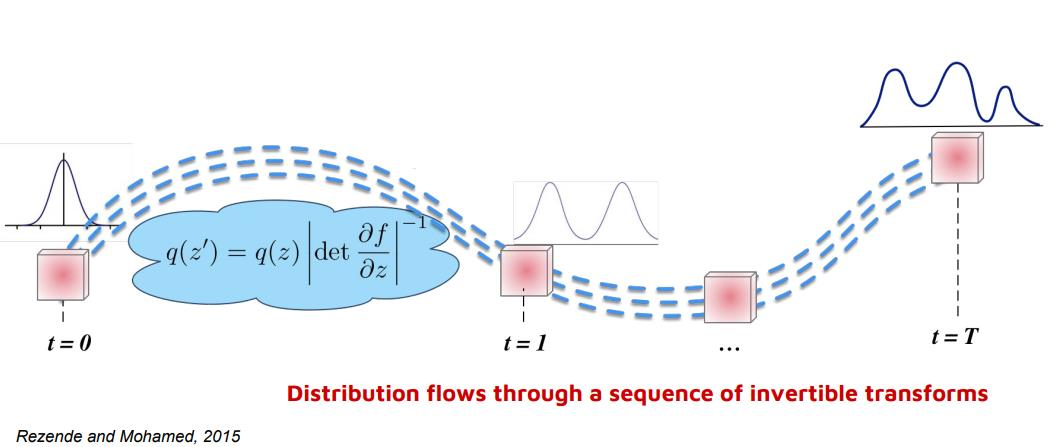
\includegraphics[width=0.7\textwidth]{fig/norm_flow.jpg}
    \caption{Normalizing Flows. See: https://www.shakirm.com/slides/DeepGenModelsTutorial.pdf}
\end{figure}

Construct a normalizing flow $\Rightarrow$ a sequence of invertible transformations that convert simple distribution to complex one. 

Invertible smooth mapping:
$f: \mathbb{R}^d\rightarrow \mathbb{R}^d$
with $f^{-1}=g$ \\
$g\centerdot f(x)=X$ if we use this to transform rv X with distribution q.
$\tilde{X}=f(x)$ have distribution. 

\textbf{(*)} $q(\tilde{x})=q(x)|det\pfrac{f^{-1}}{x}|=q(x)|det\pfrac{f}{x}|^{-1}$

Successively apply \textbf{(*)} when each map is simple. \\
$X_k=f_k \circ f_{k-1} \circ, ..., \circ f_2 \circ f_1 (X_0)$\\
So $ln(q_k(x_k))=ln q_0(x_0)-\bsum{k=1}{K}ln|det\pfrac{f_k}{x_{k-1}}|$

\begin{figure}[!ht]
    \centering
    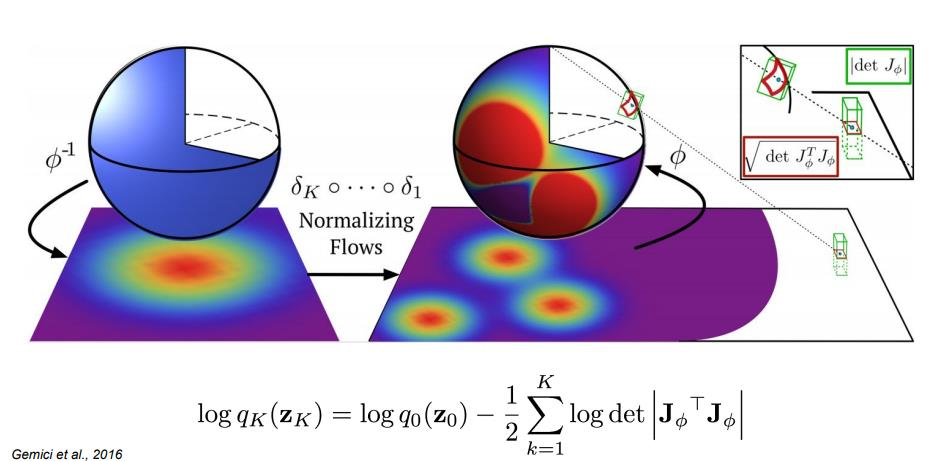
\includegraphics[width=0.7\textwidth]{fig/norm_flow_eq.jpg}
    \caption{https://www.shakirm.com/slides/DeepGenModelsTutorial.pdf}
\end{figure}

\begin{itemize}
\item The path traversed by rv $X_k=f_k(x_{k-1})$ is flow. Path successive distribution {$q_k$} is normalizing flow. 
Want inverse and Jacobian to be simple but don't want to lose expressibility. 
\item Use sequence of invertible transformations until desired complexity. 
\item Equality is by applying chain rule. 
\end{itemize}

Generative models from learning from data iid samples from P. Try to get estimate $\hat{P}$, then use it to generate new sample, rather than evaluate $\hat{P}(x)$. Often have generative model where 
$\hat{P}$ is implicit rather than explicit. Backing out $\hat{P}(x)$ is hard. 

Suppose $\hat{P}$ is defined implicitly as probability integral transform of density q by $g: \xi\rightarrow X$, so for event A: \\
$Pr[A]=Pr[g^{-1}[A]]=\int_{g^{-1}{A}}q(Z)dZ=\int_A q(g^{-1}(X))|\nabla_Xg^{-1}(X)|dX$, \\
where $\hat{P}(X)=q(g^{-1}(X))|\nabla_Xg^{-1}(X)|$ and when inverse and Jacobian are easy to compute, converting generator to density estimator easily. 

\vspace{0.5cm}
\textbf{LOTUS property}: Law of unconscious statistician.\\
$\ee[g(x)]=\sum_k g(x_k)P_x(x_k)$\\
The expectation wrt transformed density $q_k$ can be computed without explicitly knowing $q_k$. Any $\ee_{q_k}(h(x))$ can be written under $q_k$ without the need to compute the largest Jacobian term after $h(x)$.\\ 
$\ee_{q_k}[h(x)]=\ee_{q_0}[h(f_k\circ f_{k-1\circ ... \circ f_1(x_0)})]$ when $h(x)$ doesn't depend on $q_k$.

\vspace{0.5cm}
In discrete setting, change of variable formula is easier. \\
Let $x$ be discrete rv, $Y=f(x)$. The induced pmf of g is sum over inverse (???) of f:\\
$P[Y=y]=\sum_{x: f^{-1}(y)}Pr[X=x]$ where $f^{-1}(y)$ is set of all elements to $f(x)=y$. \\
f is invertible, then $P[Y=y]=P(X=f^{-1}(y))$

\vspace{0.5cm}
\textbf{Infinitesimal flows}: let the number of transformation $k\rightarrow \infty$. Describe how the initial density $q_0(x)$ evolves over time using PDE:\\
$\pfrac{}{t}q_t(x)=J_t[q_t(x)]$, $J_t$ is continuous time (???) dynamics. 

\vspace{0.5cm}
\subsection{Glow}
Let X be high-dimensional rv with unknown time distribution $X\sim P(X)$. Collect iid dataset $D$ of size $M$ and model class $P_\theta(X)$ with parameter $\theta$. 
Consider maximum likelihood, so minimize objective $\lossl(D)=\cfrac{1}{N}\bsum{i=1}{N}-logP_\theta(X^{(i)})$.

\textbf{For continuous data},\\ 
$\lossl(D)\approx \cfrac{1}{N}\bsum{i=1}{N}-logP_\theta(\bar{x}^{i})+C$, where $\bar{x}^{(i)}=x^{(i)}+u$ with $u\sim U(0,a)$, $C=Mlog\ a$, where $a$ is the quantization level. $M$ is dimension. Optimize using eg. stochastic gradient descent. 

In flow-based generation, $Z\sim P_\theta(Z)$ where Z is latent variable and $P_Z(Z)$ is simple density $X=g_\theta(Z)$ where $g_k(\centerdot)$ is invertible so $Z=f_\theta(x)=g_\theta^{-1}(x)$. \\
$f=f_1\centerdot f_2 \centerdot ... \centerdot f_k$\\
$H_0=x\overset{f_1}{\longleftrightarrow}H_1\overset{f_2}{\longleftrightarrow}H2...\overset{f_k}{\longleftrightarrow}Z=H_k$\\
$logP_\theta(x)=logP_\theta(Z)+\bsum{k=1}{K}log|det(\pfrac{H_k}{H_{k-1}})|$. \\
Easy to get Jacobian where $det(\pfrac{H_k}{H_{k-1}})$ is lower triangular. $log|det(\pfrac{H_k}{H_{k-1}})|=\sum(log|diag(\pfrac{H_k}{H_{k-1}})|)$

\begin{figure}[!ht]
    \centering
    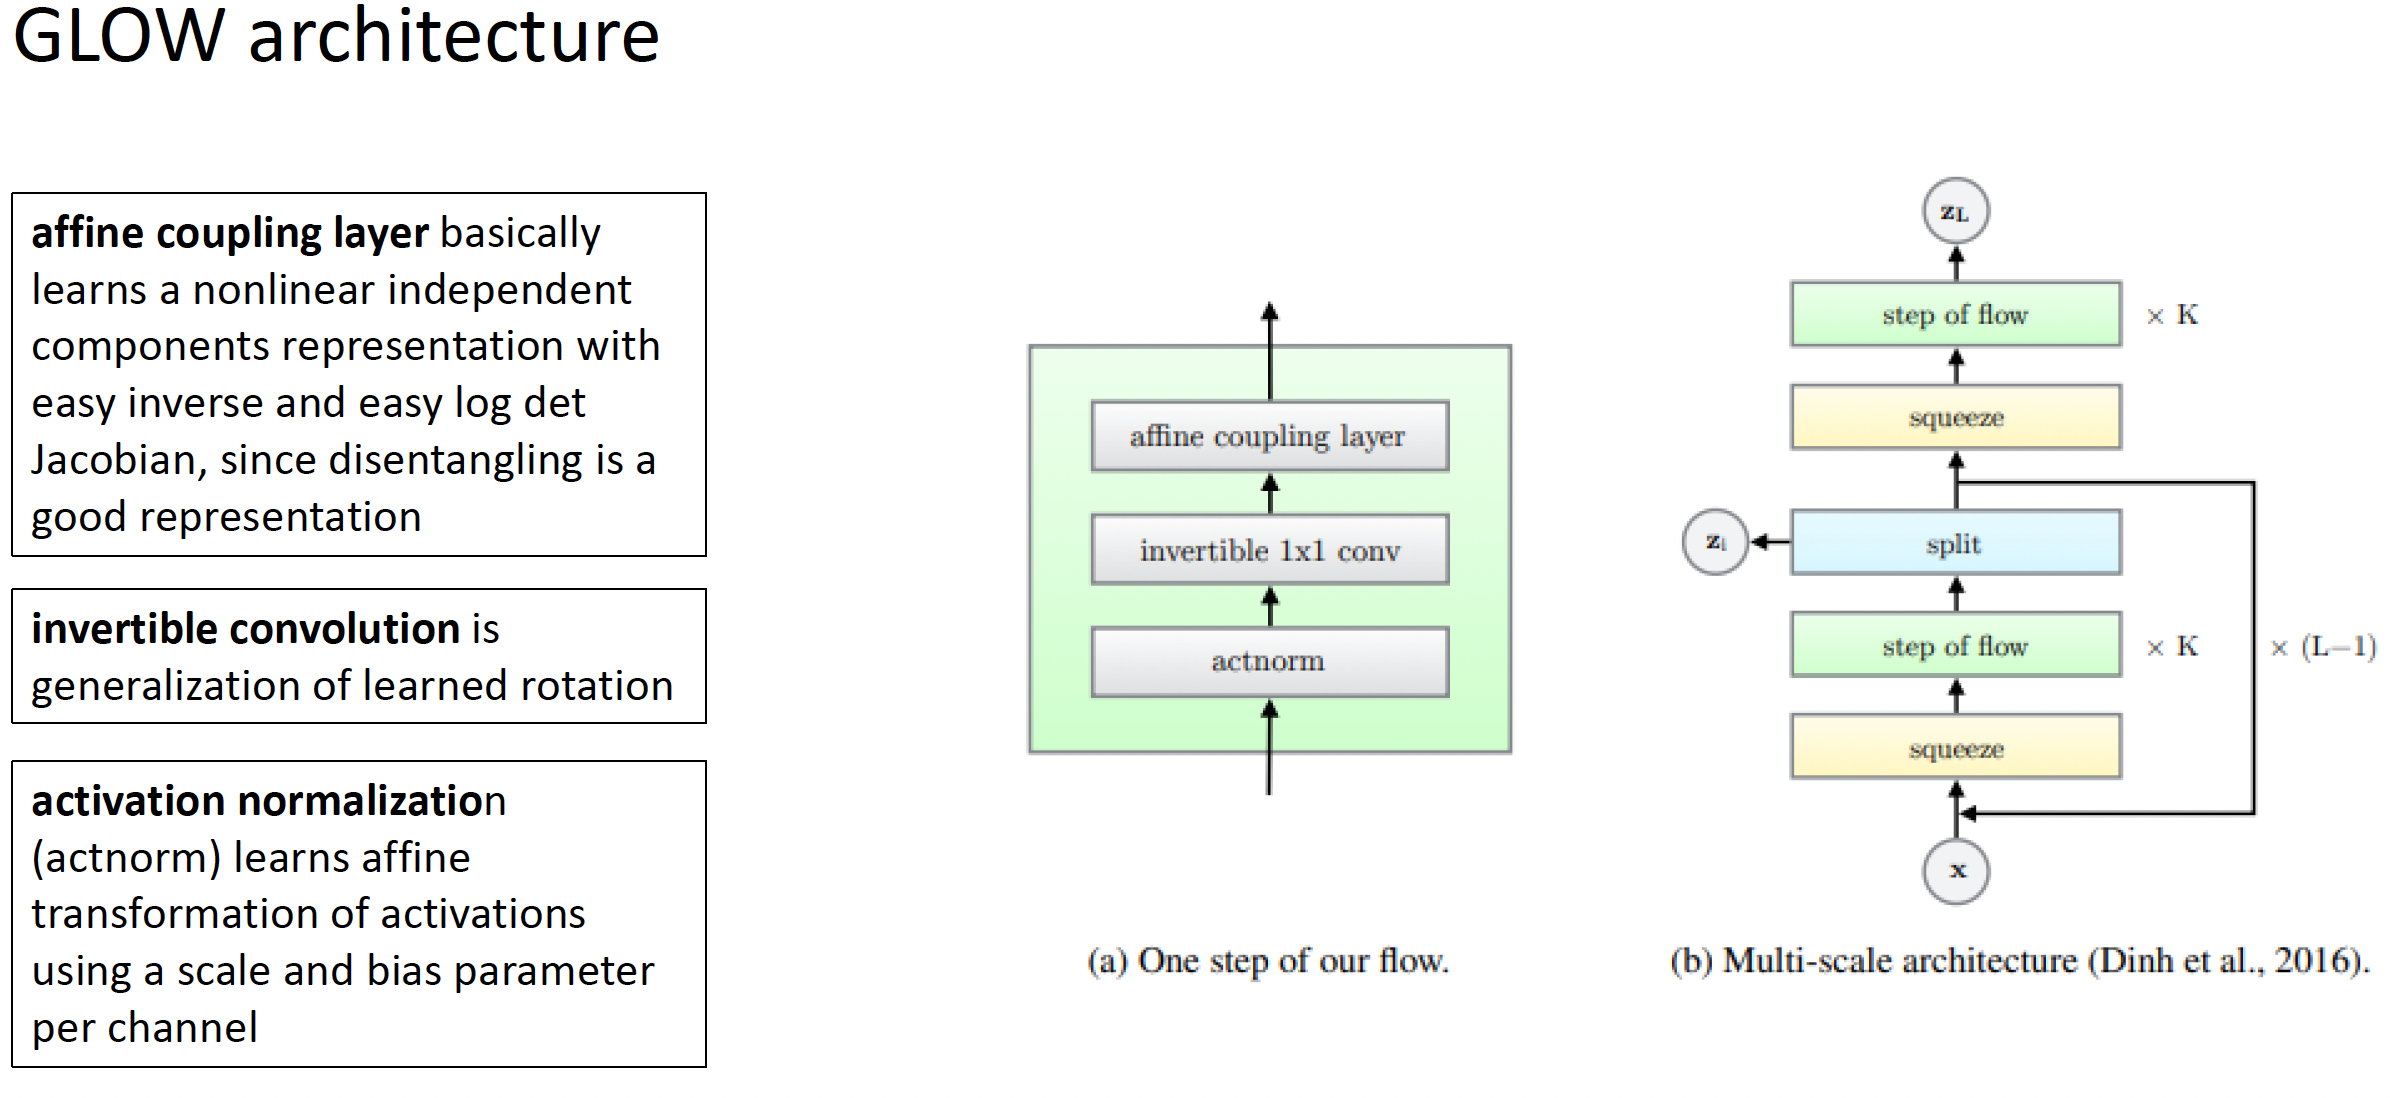
\includegraphics[width=0.7\textwidth]{fig/glow_arch.png}
\end{figure} 


\section{Lecture 4-6: Autoencoder}
\textbf{Learning objectives}:
\begin{itemize}
    \item Discuss the basic formulations and structures of autoencoders for applications in dimensionality reduction
    \item Mathematically describe why undercompleteness, contraction, and denoising might be useful ways of
    \item ucturing latent spaces
    \item Specify the deep latent variable model in the language of graphical models
    \item Describe how graphical models can be parameterized using neural networks
    \item Introduce the variational formulation of deep latent variable models 
    \item Derive ELBO (variational lower bound)
    \item Discuss how KL divergence term in ELBO determines two “distances”
    \item Derive reparameterization trick
    \item State and manipulate the InfoVAE objective
    \item Discuss some of the shortcomings of the basic ELBO-based VAE formulation
    \item Develop the basics of quantization theory
    \item Describe the VQ-VAE approach
\end{itemize}

An autoencoder is a neural network trained to attempt to copy its input to its output. Internally, it has hidden layer $h$ that describes a code or latent space used to represent the input. 

$\underset{input}{\Circled{X}}\underset{encoder}{\overset{f}{\longrightarrow}}\underset{code}{\Circled{H}}\underset{decoder}{\overset{g}{\longrightarrow}}\underset{reconstruction}{\Circled{R}}$

Tries to set $g(f(x))=x$ but are designed to be unable to learn to copy perfectly.
\begin{itemize}
    \item restricted to prevent exact copying
    \item model forced to prioritize which aspects of the input should be copied, so often learns most useful properties of data
\end{itemize}

Not just deterministic functions $f,g$, but also stochastic mappings \\
$P_{encoder}(h|x)$ and $P_{decoder}(x|h)$. 

\vspace{0.5cm}
\subsection{undercomplete autoencoders}
Constrain h to have smaller dimension than x, to force to have preserved most salient properties. \\
Reminiscent of data compression and very much a form of approximation theory. 

Learning process is minimizing loss function \\
$L(x, g(f(x)))$ where L is loss function penalizing $g(f(x))$ for lack of fidelity with x. 

When $g(\centerdot)$ fixed to be linear and L is mean-square error, an undercomplete autoencoder recovers principle components analysis (PCA), the Karhunen-Loeve transform. 

Why? When allowing nonliear (f,g), get generalization of PCA. 

One can also generalize, e.g. with sparsity autoencoder. \\
$L(x, g(f(x)))+\Omega(h)$, where $\Omega(\centerdot)$ is sparsity penalty on latent space h in addition to data fidelity term. Hopefully, this forces learning of relevant things. 

\subsection{Denoising autoencoders}
minimize $L(x, g(f(\hat{x})))$ in stead of $L(x, g(f(x)))$, where $\hat{x}$ is noisy version of x. 

DAE have to undo the noise corruption rather than simply copying, so again fry to get most informative elements. 

\subsection{Contractive autoencoders}
Different kind of regularization, to force a function that doesn't change much when x changes a little. \\
$L(x, g(f(x)))+\Omega(h, x)$ where $\Omega(h, x)=\lambda \sum_i\|\nabla_xh_i\|^2$\\ 
or $\Omega(h)=\lambda \|\pfrac{f(x)}{x}\|^2_F$ where penalty is squared Frobenius norm (sum of squared elements) of Jacobian matrix of partial derivatives associated with encoder function. 

\vspace{0.5cm}
\subsection{AE with NN}
AE used for dimensionality reduction, etc, but what about generation?

\textcircled{x} $\overset{P_{encoder}(h|x)}{\longrightarrow}$ \textcircled{h} $\overset{P_{decoder}(x|h)} {\longrightarrow}$ \textcircled{r}

Stochastic encoder/decoder. Note that $P_{encoder}$, $P_{decoder}$ don;t have to correspond to same valid joint distribution. $P_{model}(x,h)$ in fact usually don't. 

\vspace{0.5cm}
Back up to graphical models before getting to variational autoencoders (VAEs).

Consider conditional model $P_\theta(y|x)$ that approximates underlying conditional distribution $P^*(y|x)$, a distribution over variable y conditioned on input x. \\
Want to learn $P_\theta(y|x)\approx p^*(y|x)$\\
$\rightarrow$ Graphical models have an interesting calculus, e.g. Forney style graphs $\Leftrightarrow$ block diagrams. 

\textbf{Parameterizing conditional distributions with neural networks}

Differentiable feedforward neural networks are a flexible computationally-scalable kind of function approximator (universal approximation theorem). 

Learning models with neural networks with many hidden layers is deep learning. 
Notably NNs can be used to approximate pdfs and pmfs. \\
$\rightarrow$ probability models based on neural networks are computationally scalable since they allow stochastic gradient-based optimizer and scaling to large models, large datasets. \\ 
$\rightarrow$ think of them as an operator $NN(\centerdot)$

e.g. neural net can parameterize categorical distribution $P_\theta(y|x)$ over a class label y, conditioned on image x as $P=NN(x),P_\theta(y|x)=categorical(y;P)$

\vspace{0.5cm}
Consider directed graphical models that have latent variables.
$\rightarrow$ latent variables are part of model but not observed directly and not part of dataset denote by $Z$. \\
$\rightarrow$ Joint distribution $P_\theta(x,Z)$ considers observed variables and latent variables $Z$. 

A deep latent variable model (DLVM) denotes a latent variable model $P_\theta(x,Z)$ whose distributional properties parameterized by neural networks. Also conditional $P_\theta(x,Z|y)$. \\
Even when each factor (prior or conditional distribution) is relatively simple, marginal $P_\theta(x)$ can be very complex. 

A main difficulty of maximum likelihood learning in DLVMs is that marginal probability of data under model is typically intractable since $P_\theta(x)=\int P_\theta(x,Z)dZ$ may not have analytical solution or efficient estimator. 

Due to intractability, we cannot differentiate w.r.t its parameters and optimize, as we can with fully observed models (Main difficulty is posterior $P_\theta(Z|x)$). There are approximate inference techniques but ofter computationally intense. 

The framework of VAE provides a computationally efficient way of optimizing DLVMs jointly with corresponding inference model using stochastic gradient descent (SGD). 

To turn DLVM's intractable learning problem into tractable problem, introduce a parametric inference model $q_\phi(Z|x)$ which is an encoder (recognition model). $\phi$ are parameters of inference model, called variational parameters. \\
Optimize variance parameters $\phi$ such that $q_\phi=p_\theta(Z|x)$


\subsection{VAE}
Encoder has a directed graphical model, can be factorized:\\
$q_\phi=q_\phi(Z_1, ..., Z_n|x)=\prod^M_{i=1} q_\phi(Z_i|P_a(Z_i),x)$ where $P_a(Z_i)$ is set of parent of $Z_i$ in directed graph. \\
Once we have factorization $q_\phi(Z|x)$ can be parameterized using NN where $\phi$ is weights, bias of NN. 

\usefigure{fig/vae_arch.jpg}

\vspace{0.5cm}
The optimization objective of VAE is evidence lower bound (ELBO). For any choice of $\qp(Z|x)$ including choice of $\phi$\\

\begin{equation}
    \begin{split}
log \pt (x) &= \ee_{\qp(Z|x)}[log\pt(x)] \\
&=\ee_{\qp(Z|x)}[log\cfrac{\pt(x,Z)}{\pt(Z|x)}]\\
&=\ee_{\qp(Z|x)}[log \cfrac{\pt(x,Z)\qp(Z|x)}{\pt(Z|x)\qp(Z|x)}] \\
&=\ee_{\qp(Z|x)}[log\cfrac{\pt(x,Z)}{\qp(Z|x)}]+\ee_{\qp(Z|x)}[log\cfrac{\qp(Z|x)}{\pt(Z|x)}]\\
&=\lossl_{\theta,\phi}(x)+D_{KL}(\qp(Z|x)||\pt(Z|x))\\
&\Rightarrow [ELBO]\\
\end{split}
\end{equation}

where $D_{KL}$ is non-negative, so $\lossl_{\theta,\phi}=\ee_{\qp(Z|x)}[log \pt(x,Z)-log(\qp(Z|x))]\\
=log\pt(x)-D_{KL}(\qp(Z|x)||\pt(Z|x))$\\
So $\lossl_{\theta,\phi}\le log \pt(x)\Rightarrow$ lower bound of log-likelihood.

KL divergence two solutions:
\begin{itemize}
\item divergence of approximate posterior from true posterior (???).
\item gap between ELBO and $log\pt(x)$
\end{itemize}
Better approximation $\rightarrow$ higher bound.

\vspace{0.5cm}
Maximizing ELBO will optimize:\\
1. approximately maximize $\pt(x)$, so generative model is better \\
2. minimize KL divergence of approximation $\qp(Z|x)$ from $\pt(Z|x)$ so $\qp(Z|x)$ become better. \\
Jointly optimize $\phi$ and $\theta$ using SGD

\textit{Reparameterization trick}\\
For continuous latent variables and a differentiable en/decoder, ELBO can be differentiated w.r.t both $\phi$ and $\theta$ if we reparameterize. 

First, express rv $Z\sim\qp(Z|x)$ as differentiable/invertible transformation of another rv $\varepsilon$.\\
Given $\phi, x$, $Z=g(Z, \phi, x)$, $\varepsilon$ independent of x and $\phi$. \\
$\ee_{\qp(Z|x)}[f(Z)]=\nabla_\phi\ee_{p(\varepsilon)}[f(Z)]$

And since expectation and gradient commute by linearity:\\
$\nabla_\phi\ee_{\qp(Z|x)}[f(Z)]=\nabla \ee_{p(\varepsilon)}[f(Z)]=\ee_{p(\varepsilon)}[\nabla_\phi f(Z)] \approx \nabla_\phi f(Z)$\\
where we can estimate by Monte Carlo:\\
$\lossl_{\phi,\theta}(x)=\ee_{\qp(Z|x)}[log \pt(x,Z)-log \qp(Z|x)]=\ee_{p(\varepsilon)}[log \pt(x,Z)-log \qp(Z|x)]$, where $Z=g(\varepsilon,\phi,x)$. 
So we can get single Monte Carlo estimate $\hat{\lossl}_\theta p(x)$ of individual ELBO. 

\vspace{0.5cm}
\textbf{VAE problems}: 
Approximate inference distribution is often different from true posterior (from ELBO object). 

\textit{Can modify ELBO objective itself to balance correct inference and fitting training data? }

Assign some weight to balance the two parts? 
Introduce a mutual information term?  $I_{q(x,Z)}$:\\

$\lossl_{InfoVAE}=-\lambda DL(\qp(Z)||\pt(Z))-\ee_{q(Z)}[D_{KL}(\qp(x|Z))||\pt(x|Z)]+\alpha I(x,Z)\\
=\ee_{\qp(x,Z)}[log \pt(x|Z)-log \cfrac{\qp(Z)^{\lambda+\alpha-1}\pt(x)}{p(Z)^\lambda\qp(Z|x)^{\alpha-1}}]\\
=\ee_{\pt(x)}\ee_{\qp(Z|x)}[log \pt(x|Z)] - (1-\alpha) \ee_{\pt}D_{KL}(\qp(Z|x)||p(Z))-(\alpha+\lambda-1)D_{KL}(\qp(Z)||p(Z)) - \ee_{\pt}(log \pt(x))
$

\textbf{Variational Autoencoders} 
Map input to a distribution rather vector. \\
$P_\theta$ with parameters $\theta$, relationship between the input $x$ and latent encoding $Z$.\\
Prior $\pt(Z)$, likelihood $\pt(x|Z)$, posterior $\pt(Z|x)$. 

If we know actual $\theta^*$ to generate:\\
1. a sample $Z^{(c)}\sim \pts(Z)$\\
2. generate value $x^{(c)}$, $\pts(x|Z=Z^{(i)})$, $\theta^*=\argmaxp{\theta}\prod_{i=1}^n \pt(x^{(i)})$  

For computation, we approximate $\pt$ by $\qp(Z|x)$. Conditional probability $\pt(x|Z)$ is generative model. Approximate function $\qp(Z|x)$ is probalistic encoder. $\qp(Z|x)$ should be close to $\pt(Z|x)$, so minimize $D_{KL}(\qp(Z|x)||\pt(Z|x))$ 

\vspace{0.5cm}
Use more of latent code to encourage less blurring. Disentangle latent representation:\\
\textcircled{1}. Allow some Lagrangian weight between 2 ELBO terms. \\
\textcircled{2}. introduce a mutual information term. 

\begin{figure}[!ht]
    \centering
    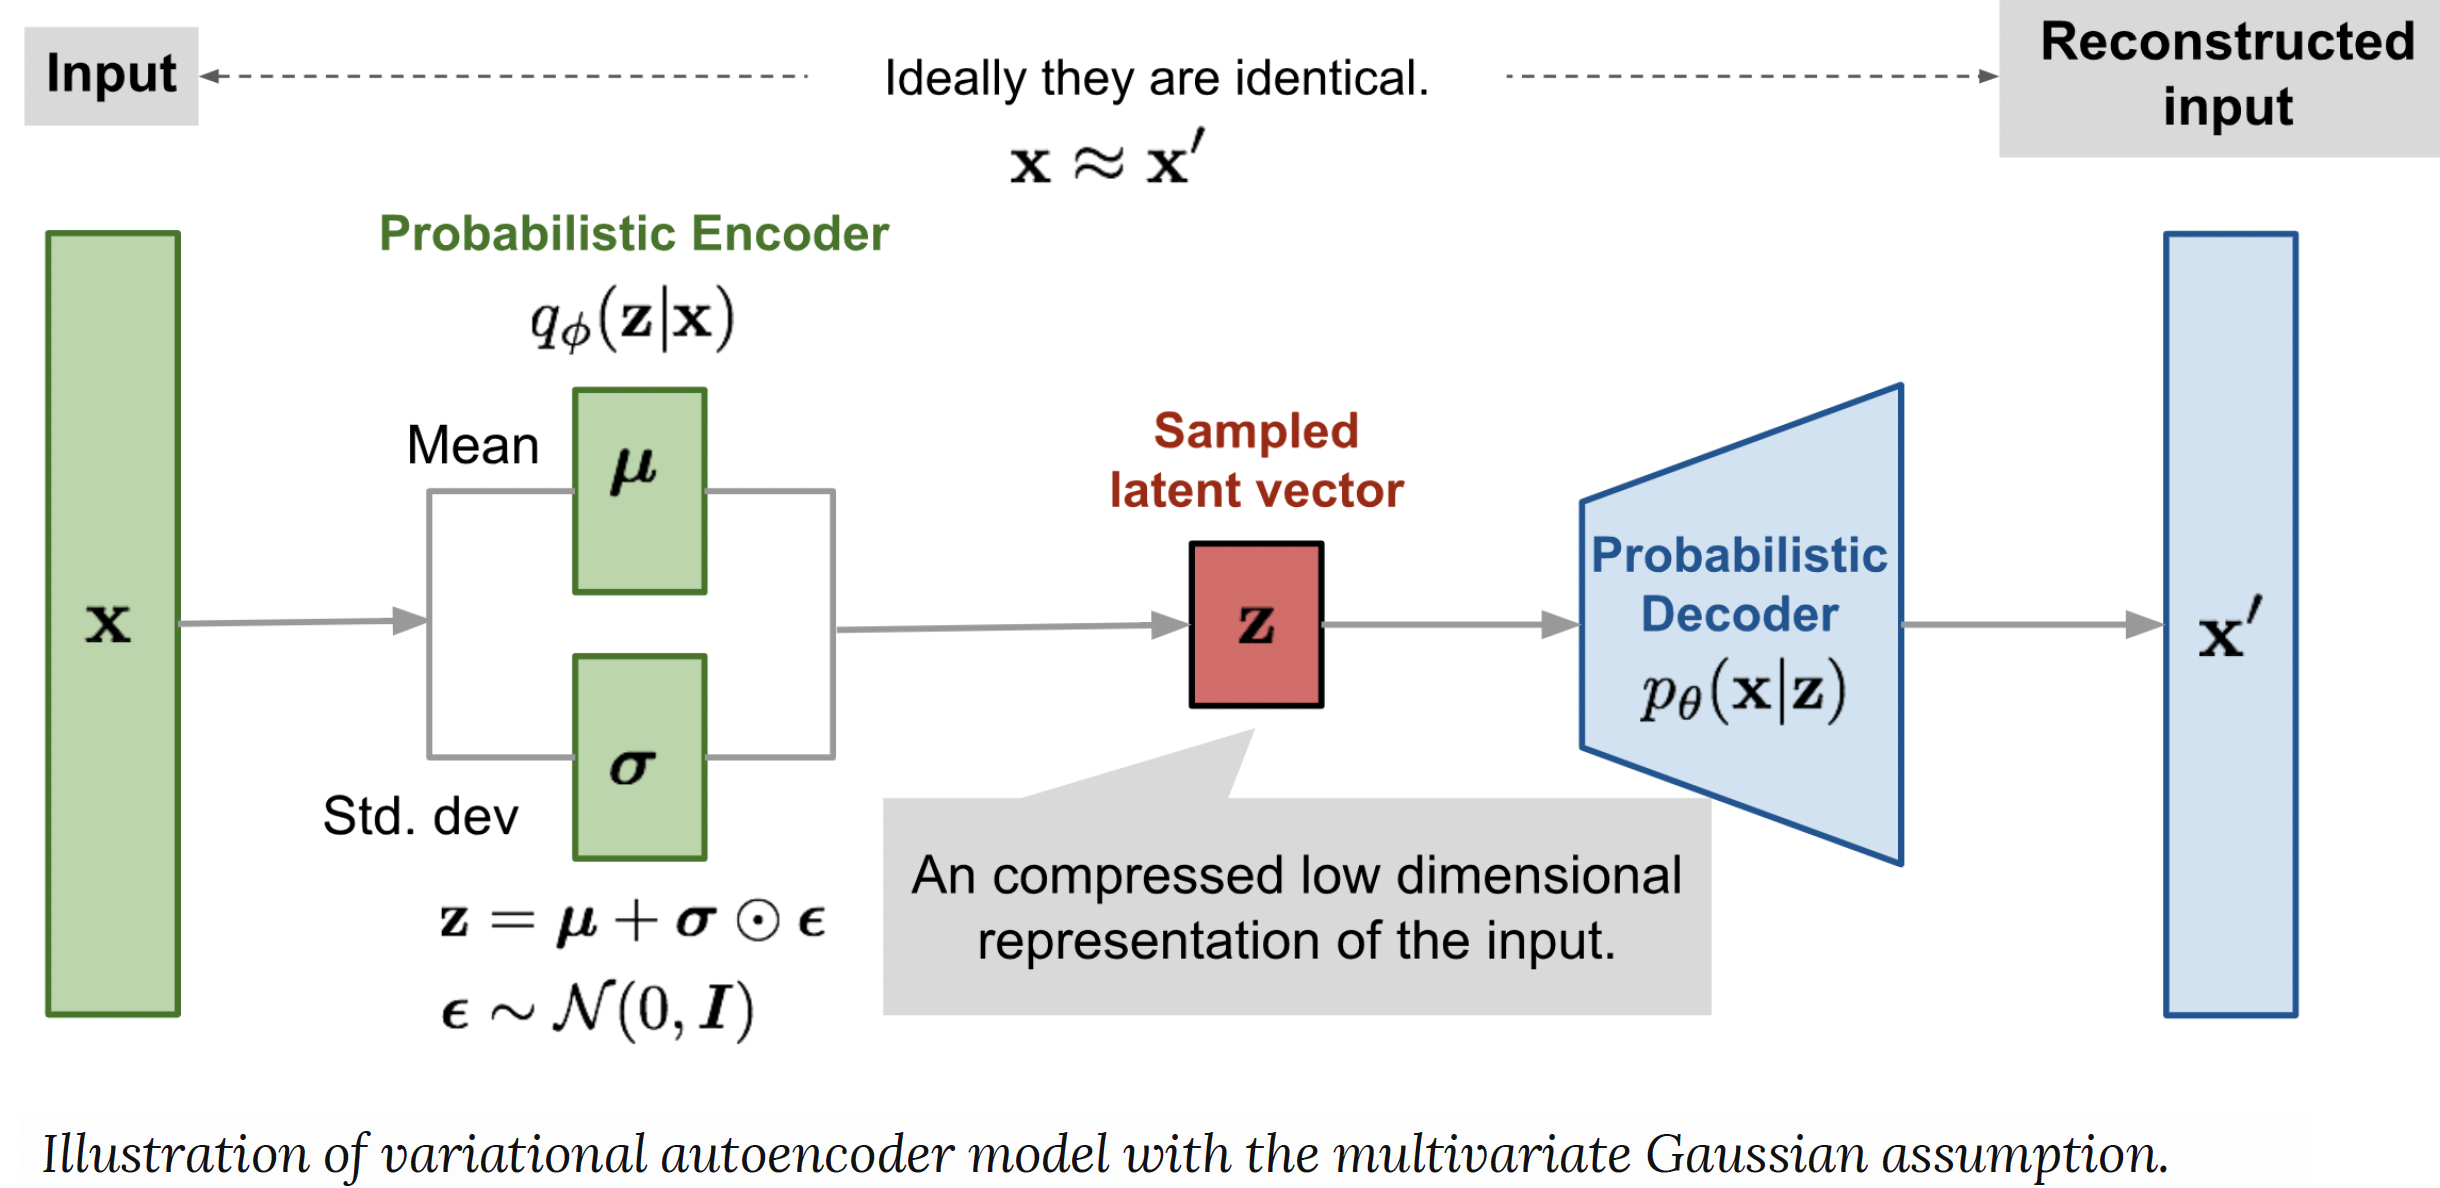
\includegraphics[width=0.7\textwidth]{fig/vae.png}
\end{figure}

\textbf{Vector quantized VAE(VQ-VAE)}
Constrain latent space to discrete. 

\textit{Introduction to quantization:} \\
Consider iid sequence of analog rv $v_1, v_2\sim P_U(u)$ quantizer maps this sequence into a sequence of discrete rv $v_1,v_2,...$. If restrict to alphabet of size $M$, then $v_M$ can't represent $V_M$ perfectly on general, larger $M$ implies less distortion. 

$V_m\longrightarrow \fbox{encoder} \overset{I\leftarrow\{1,...,M\}}{\longrightarrow} \fbox{decoder} \longrightarrow V_m$

Mean-squared distortion is $\ee[(u-v)^2]$

\vspace{2cm}
\begin{figure}[!ht]
    \centering
    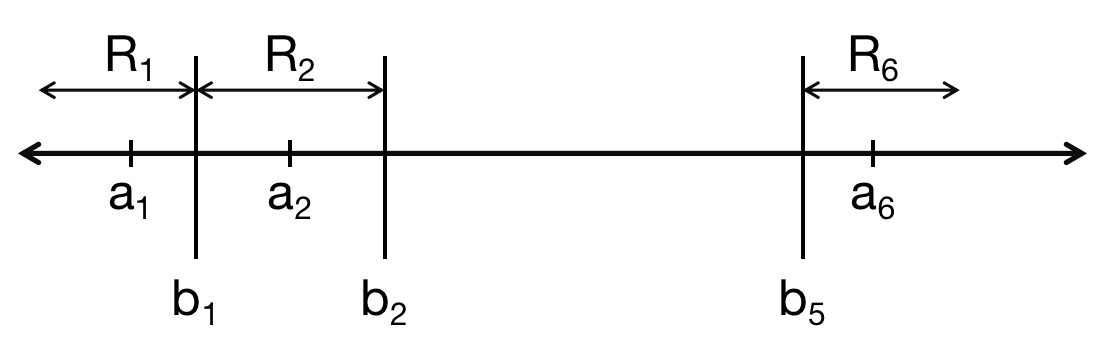
\includegraphics[width=0.7\textwidth]{fig/vae_quant.png}
\end{figure}

\begin{itemize}
\item Given representation points $\{a_j\}$, how should intervals $\{R_j\}$ chosen? \\
Nearest neighbor condition, $b_j=\cfrac{a_j+a_{j+1}}{2}$
\item Given intervals $\{R_j\}$, how should representation points $\{a_j\}$ be chosen? \\
$a_j=\ee[V|V\in R_j]$
\end{itemize}

\textit{Lloyd-Max algorithm:}\\
Given M, $f_u(U)$;\\
\textcircled{1}. Choose arbitrary initial set of M representation points, $a_1>a_2<...<a_M$\\
\textcircled{2}. for each j, $b_j=\cfrac{a_j+a_{j+1}}{2}$\\
\textcircled{3}. for each j, set $a_j=\ee[V|V\in [b_{j-1}, b_j]]$\\
\textcircled{4}. Repeat \textcircled{1},\textcircled{2} until MSE doesn't change.

\vspace{0.5cm}
Vector quantization
Quantize n rv together. Region $R_j$ must be set of points that are closest to ($a_j, a_j$), then to any other representation points.

Varanoi regions: \\
Convex polygonal regions; boundaries are perpendicular; bisectors between neighboring parts. 

\begin{figure}[!ht]
\centering
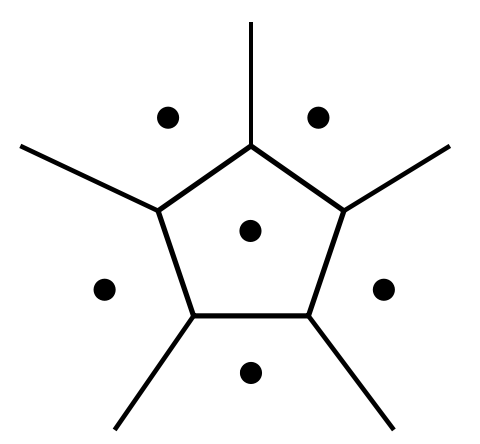
\includegraphics[width=0.4\textwidth]{fig/convex_poly_region.png}
\end{figure}

\textbf{VQ advantages}:\\
1. space filling; 2. shape; 3. memory

VQ-VAE encoder which parameterize approximate posterior $q(Z|x)$ decode $p(x|Z)$ prior $p(Z)$. 

Define latent embedding space as subset of $R^D$ with k representation points, $e_i\in \mathbb{R}^D, i=1,...,k$.

The encoder output $Z(x)=Z_e$ goes through nearest neighbor. Look up to match one of the k embedding vectors and then this input to decoder $D(\centerdot)$.

$Z_q(x)=quantize(E(x))\centerdot e_k$, where $k=argmin\|E(x)-e_i\|_2$. For training, since argmin not differentiable in discrete case, gradient of loss function $\nabla_Z L$ from discrete input $Z_q$ copy to encoder output. 

Consider 3 terms in loss: \\
1. Reconstruction loss, which optimizes encoder/decoder\\
2. Due to copying from $Z_e$ to $Z_q$, need something to form VQ \\
3. Ensure encoder commits to a representation

Let $sg(\centerdot)$ be stop gradient, defined as identity of forward computation and has $D$ partial derivatives:\\
$L=\underset{reconstruction\ loss}{\|x-D(e_k)\|^2_2} + \underset{VQ\ loss}{\|sg[E(x)-e_k]\|^2_2 }+ \underset{constraint\ loss}{\beta\|E(x)-sg(e_k)\|_2^2}$

Let piece is learn a prior in latent space $P(Z)$, so we can sample from it to do generalization via decoders. 

\section{Lecture 7-9: generative adversarial networks (GANs)}
\textbf{Learning objectives}:

\begin{itemize}
\item Explain the basic game-theoretic formulation of GANs
\item Define a normal form game
\item Describe the standard cost functions for generators and discriminators in GANs
\item Describe the cost functions for generators and discriminators in GANs that lead to MLE
\item Derive cost functions for generators and discriminators in GANs that lead to MLE
\item Discuss stochastic gradient descent algorithms for GANs
\item Describe the mode collapse and partial mode collapse phenomena and several ways to mitigate it
\item Describe the basic formulation of Wasserstein GANs
\item Derive the Kantorovich-Rubinstein duality in optimal transport theory
\item Discuss f-GANs
\item Describe GANs in the robust statistics framework
\item Discuss novelty-quality tradeoffs in creativity
\item Discuss ways that have been proposed to assess the performance of generative algorithms, especially GANs which only have implicit density estimation, and how this is related to interpolative and extrapolative generation
\end{itemize}

One weakness of VAE is the variational bounds has a gap such that the model will not be consistent. GAN approach differently circumvents needs for variational bound $\Rightarrow$ NN models within GAN are universal approximators, and this enables a proof of asymptotic consistency in getting true objective distributions.

Training requires finding Nash equilibrium of a game, which is in general more difficult than optimizing an objective function. \\
Generator creates sampler that are intended to come from same distribution as training data\\ 
Discriminator examines samples to determine whether real or fake (supervised learning for binary classification).

In graphical model form of GAN, there will be observed variable $X$ and latent variable $Z$. The players in game are represented by 2 functions, that one differentiable w.r.t their inputs and their parameters. 

Discriminator is function $D$ that takes x as input has parameters $\dt$; generator is function that takes Z as input with parameters $\gt$. 
Both players have cost functions that are defined in terms of both player's parameters. 

Discriminator wants to minimize $\jd(\dt,\gt)$, only controls $\dt$. Generator wants to minimize $\jg(\dt,\gt)$, only controls $\gt$. 
Each player's cost depends on other player parameters $\Rightarrow$ Game, rather than optimization. 

\begin{figure}[!ht]
    \centering
    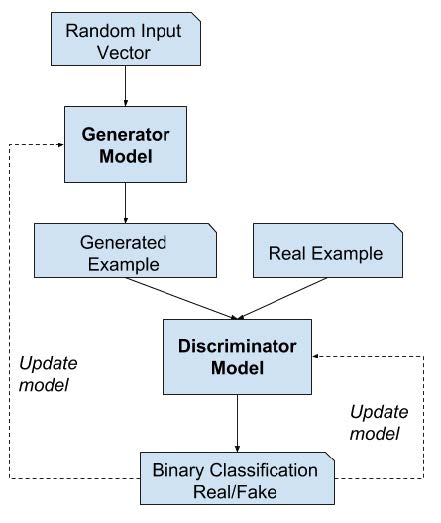
\includegraphics[width=0.5\textwidth]{fig/gan_arch.jpg}
    \caption{GAN architecture}
\end{figure}

\vspace{0.5cm}
\subsection{Nash Equilibrium}
a tuple $(\dt, \gt)$ is local minimum of $\jd$ w.r.t. $\dt$ and is local minimum $\jg$ w.r.t $\gt$. 

Normal form games: An N-player normal form game consists of:\\
1. finite set of N players\\
2. strategy spaces for players, $S_1, S_2, ..., S_N$\\
3. payoff function for players, $U_1: S_1\times S_2\times...\times S_N\rightarrow \mathbb{R}$

A natural representation of a two-player game is using a bi-matrix colum strategy.

\begin{center}
\begin{tabular}{c | c}
    & column strategy \\
    \hline 
    row strategy & $\vecb{(u_1(r_1,c_1), u_2(r_1,c_1))&(u_1(r_1,c_2), u_2(r_1,c_2))&...\\
    (u_1(r_2,c_1), u_2(r_2,c_1)) & ... & ...\\
    ... & ... & (u_1(r_m,c_n), u_2(r_m,c_n))
    }$\\
\end{tabular}
\end{center}

where $s_1=\{r_i, i=1,2,..m\}$, $s_2=\{c_j, j=1,...,n\}$

Proofs of existence of Nash equilibrium come from fixed point theorems like Bronwer, Kakutari, etc. 

Training process consists of simultaneous SGD $\Rightarrow$ in each time step, two datasets sampled: \\
\textcircled{1}. subset of x, training data\\
\textcircled{2}. set of z values drawn from current models prior over latent variables.

Two simultaneous gradient steps:\\
One updates $\dt$ to reduce $\jd$\\
One updates $\gt$ to reduce $\jg$

Cost function for discriminator for binary classification. \\
$\jd(\dt,\gt)=\mhalf \ee_{x\sim \pdata{x}}logD(x)\mhalf\ee_Zlog(1-D(G(Z)))$

Cross entropy cost to minimize to train standard binary classification. with a sigmoid output. 

By training discriminator, we can also estimate $\cfrac{\pdata{x}}{\pmodel{x}}$. Estimating this ratio allows computing various divergences. 
Rather than lower bounds like ELBO, GAN approximation based on using supervised learning to estimate ratio of two densities. 

\vspace{0.5cm}
\textit{What's cost function for generator?}\\
Simplest approach is to require game to be zero sum, so sum of costs of all players is 0. $\jg=-\jd$. 

So entire game can be summarized by value function specifying the discriminator's payoff: \\
$V(\dt,\gt)=-\jd(\dt,\gt)$

Since zero sum games yield minmax characterization: \\
${\gt}^* =\argminp{\gt}\ \underset{\dt}{max}V(\dt,\gt)$, where ${\gt}^*$ corresponding to minimizing Jenson-Shanon (JS) divergence between data and model distribution.

An alternative heuristic that seems to work better in practice $\Rightarrow$ still use cross entropy minimization for generator, but instead of flipping sign on discriminator, we flip the target used to construct cross entropy. \\
$\jg=\mhalf \ee_Z logD(G(Z))$. 

So generator maximizing the log-probability of discriminator being mistaken rather than minimizing log probability of discriminator  being correct.

\vspace{0.5cm}
\textbf{Maximum likelihood}

MLE is minimizing KL divergence. \\
$\Theta^*=\argminp{\theta}D_{KL}(\pdata{x}||\pmodel{x,\theta})$

If discriminator optimal, then we can minimize to obtain MLE when\\ 
$\jg=\mhalf\ee_Z\ exp(\sigma^{-1}(D(G(Z))))$, where $\sigma$ is logistic sigmoid. 

\fbox{ minmax $\Leftrightarrow$ JS \& MLE $\Leftrightarrow$ KL}

\vspace{0.5cm}
Goals of discriminator is to minimize: \\
$\jd(\dt,\gt)=\mhalf \ee_{x\sim \pdata{x}}logD(x)-\mhalf \ee_Z log(1-D(x))$ w.r.t $\dt$

Value for $D(x)$ is specified for each value x to minimize $\jd$ w.r.t D.
Write functional derivatives for a given x, set it zero: 
$\pfrac{\jd}{D(x)}=0$. Solving will yield $D^*(x)=\cfrac{\pdata{x}}{\pdata{x}+\pmodel{x}}$

\usefigure{fig/gan_ratio_density.jpg}

\vspace{0.5cm}
MLE:\\
$\pfrac{\jg}{G}=\ee_{x\sim p_g}f(x)\pfrac{log(P_g(x))}{G}$, where we assumes:\\
1. $P_g(x)\geq 0$ everywhere, so $P_{g(x)}=exp(log(P_g(x)))$\\
2. function derivative is continuous, so we can interchange derivative integral (Leibniz rule)

So we see derivatives of $\jg$ are close to what we want, just expectation is w.r.t samples from $\P_g$ rather that $P_{data}$, so pick $f(x)=\cfrac{\pdata{x}}{P_g(x)}$ by importance sampling trick. 

GAN is zero sum mimax game with \textcircled{1} discriminator \textcircled{2} generator. Most people think GAN successful if:\\
1. generator reliably generates data that fools discriminator\\
2. creates sample that are as diverse as distribution of real world

\usefigure{fig/good_gan.jpg}

\usefigure{fig/gan_metric.jpg}

\textbf{Model collapse}

Fail to achieve \textcircled{2} by achieving \textcircled{1} through a concentrated distribution. Model collapse may arise because maxmin solution of GAN game is different from minmax solution. 

When we find model $G^*=\underset{G}{min}\underset{D}{max} V(G,D)$, $G^*$ will draw sample from the full distribution when we exchange order to have maxmin $G^*=\underset{D}{max}\underset{G}{min} V(G,D)$.
Min of G is inner loop of optimization. The generator asked to map every Z value to the single output x that the discriminator believes is most to be real rather than fake. 

Simultaneous gradient descent doesn't clearly privilege minmax over maxmin. 

\textbf{Unrolling}: updating generator's loss function to backpropagate through k steps of gradient updates for discriminator. Let generator see k steps into future to encourage more diverse samples. 

\textbf{Parking}: modify discriminator to make decisions on several samples of same class, either real or fake. Seeing multiple identical cases is give a way (???) for fake.

\usefigure{fig/model_collapse.jpg}

\subsection{Wasserstein Loss}
Formulate loss functions to more directly represent minimizing distance between two probability distributions.\\
$\Rightarrow$ Make a winning turn in the game correlate with actually reducing distance between $P_g$ and $P_{data}$ rather than just fooling discriminator. 

Recall JS divergence, $JS(P||Q)=\cfrac{1}{2}D_{KL}(P||M)+\cfrac{1}{2}D_{KL}(M||Q)$, where $M=(P+Q)/2$ was implicit objective in original GAN. 

Now consider Wasserstein distance instead (optimal transportation theory):\\
$W(P,Q)=\underset{\delta\in \Pi(P,Q)}{inf}\ \ee_{(x,y)\sim \delta}[\|x-y\|]$, where $\Pi(P,Q)$ is a set of all joint distribution with marginal P, Q, $\delta(x,y)$ is amount of mass that must be moved from x to y to convert P to Q. 

Wasserstein distance is the cost of optimal transport map\\
$\Rightarrow$ continuous almost differentiable everywhere\\
$\Rightarrow$ JSD locally saturates as discriminator gets better, so gradients become zero and vanish. 

\vspace{0.5cm}
Hard to handel inf, we can use Kantorovich-Rubirstein duality.\\
$W(P,Q)=\underset{\|f\|_L\le 1}{sup} \ee_{x\sim P}[f(x)]-\ee_{x\sim Q}[f(x)]$, where sup is over all 1-Lipshitz continuous functions. 

K-Lipshitz continuity: given metric spaces $(x,dx), (y,dy)$, map $f: x\rightarrow y$ is k-Lipshitz if $dy(f(x_1), f(x_2))\le k dx(x_1, x_2)$ for all $(x_1, x_2)\in X$


\vspace{0.5cm}
\underline{Proof of K-R duality}\\
Introduce Lagrangian multipliers $f,g: \lambda\rightarrow R$ (bounded measurable):\\ 
\begin{equation}
    \begin{split}
\lossl(\delta, f,g)& =\int_{X\rightarrow x} \|x-y\|^2 \delta(x,y)dydx-\int_X(P(x)-\int \delta(x,y)dy)f(x)dx-\int_x(q(y)-\int(x,y)dx)g(y)dy\\
\lossl(\delta, f, g) &= \ee_{x\sim P}[f(x)]+\ee_{y\sim q}[g(y)] +\int_{X\rightarrow x} (\norm{x-y}-f(x)-g(y)) \delta(x,y) dydx \\
W(P, P_g) &=\underset{\delta}{inf}\ \underset{f,g}{sup} L(\delta,f,g) = \underset{f,g}{sup}\ \underset{\delta}{inf} L(\delta, f,g)
    \end{split}
\end{equation}

Note if $\norm{x-y}<f(x)+g(y)$ for some $x,y\in X$, then we can concentrate mass of $\delta$ at $(x,y)$ and sent $\lossl (\delta, f,g)\rightarrow -\infty$, so for all x, y, we must have $f(x)+g(y)\le \norm{x-y}$

Best we can do is minimize $\delta$ over $\delta=0$\\
$\underset{f,g}{sup}\ \underset{\delta}inf\ \lossl(\delta, f,g)=\underset{f,g,f(x)+g(y)\le \norm{x-y}}{sup} [\ee_{x\sim p}[f(x)]+\ee_{y\sim q}[g(y)]]=W(p,q)$

Observe that optimizing over class of 1-Lipshitz function is lower bound on Wasserstein. 

If h is 1-Lipshitz,\\
$\ee_{x\sim p}[h(x)]-\ee_{y\sim q}[h(y)]=\int_{X\sim x}(h(x)-h(y))\delta(x,y)dxdy\\
\le \int_{X\sim x}\norm{x-y}\delta(x,y)dxdy\\
\le W(p,q)$

$\Rightarrow \underset{\|h\|_L\le 1}{sup}[\ee_{x\sim p}[h(x)-\ee_{y\sim q}[h(y)]]]\le W(p, q)$. 
Wants to show this holds with equality. 

Consider a function $\mathcal{K}$ defined as:\\
$\mathcal{K}: x\rightarrow \underset{u}{inf}[\|x-u\|_2-g(u)]$, since g is bounded, inf is finite, and $\mathcal{K}$ is well-defined.

\textbf{Claim}: $\mathcal{K}$ is 1-Lipshitz\\
\underline{Proof}: given $x,y\in X$. For any $u\in X$, by triangular inequality:\\
$\mathcal{K}(x)\le \norm{x-u}-g(y)\le \norm{x-y}+\norm{y-u}-g(u)$\\
This holds for any u, $\mathcal{K}(x)\le \norm{x-y}+\underset{u}{inf} [\norm{x-u}-g(u)]=\norm{x-y}+\mathcal{K}(y)$\\
$\mathcal{K}(x)-\mathcal{K}(y)\le \norm{x-y}$, exchange x,y\\
$|\norm{\mathcal{K}(x)-\mathcal{K}(y)}|\le \norm{x-y}$. It's 1-Lipshitz. 

For any f, g that satisfy $f(x)+g(y)\le\norm{x-y}$,\\ 
$f(x)\le \mathcal{K}(x)\le \norm{x-x}-g(x)=-g(x)$

Plugin in: $\ee_{x\sim p} +\ee_{y\sim q}[g(y)] \le \ee_{x\sim p}[\mathcal{K}(x)]-\ee_{y\sim q}[\mathcal{K}(y)]$

We conclude\\
$W(p,q)=\underset{f,g,f(x)+g(y)\le \norm{x-y}}{sup}[\ee_{x\sim p}[f(x)]+\ee_{f\sim q}[g(y)]]
\le \underset{\norm{w}\le 1}{sup}[\ee_{x\sim p}[h(x)]-\ee_{y\sim q}[h(y)]]\le W(p,q)$

End of proof. 

\vspace{0.5cm}
Objective of generator $\Rightarrow$ minimize Wasserstein distance rather than fooling discriminator. 

\subsection{f-GAN}
Have different f-divergences as their objective. 

Let P, Q be defined over the same space $P<<Q$ (P is absolutely continuous w.r.t Q), then for a convex function $f: f(1)=0$, f-divergence of P from Q:\\
$D_f(P||Q)=\int f(\cfrac{dP}{dQ})dQ$. 

When both absolutely continuous w.r.t a common reference measure (Lebesgue measure).\\
$D_f(P||Q)=\int f(\cfrac{p(x)}{q(x)})q(x)dx$ \\
1. if $f(t)=tlog\ t\Rightarrow$ KL divergence.\\
2. if $f(t)=\cfrac{1}{2} [(t+1)log\ \cfrac{2}{t+1}+tlog\ t]\Rightarrow$ JS. 

We can put in f-divergence as objective to define f-GAN. Match distribution as design idea, "density approximation".

\vspace{0.5cm}
\textbf{Reformulation of GANs in robust statistics framework}

Picking a generator $g(\centerdot)$ for $\mathcal{Y}$, minimize loss $\lossl(P_{g(Z)}, P_x)$ over all $g\in \mathcal{Y}$\\
$\lossl(P_{g(Z)},P_x)$ to be small. If $\lossl$ and $\mathcal{Y}$ don't get right kind of small, try something else. 

How to have $P_x$ to be a slight perturbation of $g\in \mathcal{Y}$ under $\lossl$ that make sense?

\section{Lecture 10-11: Auto regressive model}
\textbf{Learning objectives}:

\begin{itemize}
\item Walk through Markov approximations of language
\item Discuss generative grammar formulations of language and their contrast with Markov models
\item Draw out autoregressive models parameterized by neural networks, including those with causal convolution layers
\item Discuss MLE for autoregressive models
\item Derive the innovations form of random processes that meet the Paley-Wiener conditions and interpret in terms of convolutions
\item Show the relationship between minimum mean-squared estimation and maximum entropy extrapolation
\item Further discuss neural network-based autoregressive models
\end{itemize}

$P(x,y)=P(x|y)P(y)=P(y|x)P(x)$, $P(x)=\sum_yP(x,y)$ 

Broadly, we want to model some $P(x)$. We hypothesize some factored form. \\
First, we generally write $P(x)$ for $x\in X^D$. e.g. $X=\{a,b,...,z\}$ or $x=\{1,2,...,256\}$.\\
$P(x)=P(x_0)\prod_{d=2}^D P(x_d|x_{<d})$, $x_{<d}=\{x_1,...,x_{d-1}\}$. e.g. $P(x)$ for $D=3$, $P(x_1)P(x_2|x_1)P(x_3|x_1,x_2)$. This is too computation heavy. 

To help, we consider auto regressive models:\\
1. finite memory; 2. approximation; 3. shared parameters (NN)

\textbf{Finite memory}: \\
$P(x_1)P(x_2|x_1)\prod_{d=3}^D P(x_d|x_{d-1},x_{d-2})$, then also use a small multilayer perceptron to model the parameters. Single shared MLP to prevent the probability for $x_d$. 

\usefigure{fig/ar_mlp.png}

\textbf{Long range memory}: \\
Recurrent neural network. Make conditional distribution of form $P(x_d|x_{<d})=P(x_d|RNN(x_{d-1},h_{d-1}))$ where $h_d=RNN(x_{d-1},h_{d-1})$ and $h_d$ is hidden content that act as memory to capture long-range content. 

\usefigure{fig/ar_rnn.png}

\textbf{issue}: \\
They are sequential, slow in training/inference. Numerical issues in training them. 

\textbf{Conditional neural network}: can be used to model long-range dependencies rather than RNN. Advantages:\\
1. kernels are shared (efficient parameterization)\\
2. processing in parallel (speedy computation) \\
3. stacking more layers allows effective kernel size to grow with network depth. 

\vspace{0.5cm}
\textbf{Discrete time random process}:\\
One view of auto-regressive models is that they are predictors connect back to classic work in random process. 

$x[n]$ is a sequence of random variables, defined for indices $n=-\infty,...,0,1,2,...$, \\
$\Omega\rightarrow x[n]$, $\Gamma(z)=\cfrac{1}{L(z)}$

A discrete-time system is minimum phase if its system $L(z)$ and its inverse $\Gamma(z)$ are analytic in the exterior of unit disk $|z|>1$. 

A real wide-sense stationary digital process is regular if it's power spectrum:\\
$\{S(z)=\bsum{m=-\infty}{\infty} R[m]z^{-m}\}$, where $R[m]$ is autocorrelation and this is Z transform. 

Can be written as a product: $S(z)=L(z)L(\cfrac{1}{z})$. 
Denote by $l(n)$ and $\gamma[n]$, the delta response of $L(z)$ and $\Gamma(z)$. 

\vspace{0.5cm}
\textbf{Whiken process}:\\
We can conclude that a regular process $x[n]$ is linearly equivalent with a whik-noise process $i[n]$:\\
$i[n]=\bsum{k=0}{\infty}\gamma[k]x[n-k]$, where $R_{L1}=\delta[m]$\\
$x[n]=\bsum{k=0}{\infty}l[k]i[n-k]$, where $\ee[x^2[n]]=\bsum{k=0}{\infty}l^2[k]<\infty$

$x[n] \longrightarrow $\fbox{$\Gamma(z)$} $\overset{i[n]}{\longrightarrow}$ \fbox{$L(z)$} $\longrightarrow x[n]$

The process $i[n]$ is the innovation sequence of $x[n]$, and $L(z)$ is its innovations filter. 
The whikening filter of $x[n]$ is $\Gamma(z)=\cfrac{1}{L(z)}$. H can be shown that the power spectrum $S(z)$ of a process $x[n]$ can be factored as $S(z)=L(z)L(\cfrac{1}{z})$ if it satisfies Paley-Wipper condition (P-W condition).

\vspace{0.5cm}
\textbf{P-W condition}:

$\bint{-\pi}{\pi}|logS(w)dw|< \infty$. If power spectrum $S(w)$ is integrable function, the P-W condition reduces to $\cfrac{1}{2\pi}\bint{-\pi}{\pi} lnS(w)dw>-\infty$

\vspace{0.5cm}
\textbf{Auto-regressive}

The process $x[n]$ is called autoregressive (AR) if $\lossl(z)=\cfrac{b_0}{1+a_1z^{-1}+...+a_nz^{-n}}$ and so process $x[n]$ satisfies recursion \\
$x[n]+a_1x[n-1]+...+a_Nx[n-N]=b_0i[n]$ where $i[n]$ is whik-noise process. 

The past $x[n-N]$ of $x[n]$ only depends on the past of $i[n]$ where $\ee[i^2[n]]=1$

\textit{Estimation/prediction of AR processes}: \\
Suppose $s[n]$ is an AR process of order M with autocorrelation $R[m]$. $\bar{S}[m]$ is some other general process with autocorrelation $\bar{R}[m]$, s.t. $\bar{R}[m]=R[m]$ for $|m|<M$. 
The predictor (MSE optimizing) for these two process of order M util be identical, because they depend only on $R[m]$ for $|m|<M$.

Consider a class $C_M$ of processes with identical autocorrelation for $|m|<M$, each $R[m]$ is an extrapolation of given data, and it can be shown the extrapolating sequence, obtained using maximum entropy, method is autocorrelation of an AR process of order M. 

So maximum entropy extrapolation is autocorrelation of $S[n]\leftarrow C_m$ where optimized predictor maximize the minimum MSE. \\
Max entropy $\Leftrightarrow$ MMSE prediction

\vspace{0.5cm}
\textbf{Deep generative AR models}

Think of x the thing we are modeling as categorical\\
$x=\{1, ..., 256\}^{256\times 256}$

We model $P(x)$ using the casual convolution-type architecture with many layers. Each conditional as follows:\\
$P(x_d|x_{<d})=categorical(x_d|\theta_d(x_{<d}))=\prod_{l=1}^L (\theta_{d,l})^{x_d=l}$, where $[a=b]$ is Iverson bracket notation:
\begin{equation*}
\begin{cases}
[a=b]=1 & if\ a=b\\
[a=b]=0 & if\ a\neq b\\
\end{cases}
\end{equation*}

and $\theta_d(x<d)$ is the output of the casual convolution layer with softmax in last layer, so $\bsum{l=1}{L}\theta_{d,l}=1$

\usefigure{fig/ar_causal_conv.png}

\vspace{0.5cm}
\textit{What should be training objective?}

we can maximize log-likelihood $ln\ P(D)$ where D is iid dataset of $\{x_1,...,x_N\}$. So\\
\begin{equation*}
    \begin{split}
max\ lnP(D) &= ln\prod_nP(x_n)\\
&=\bsum{n}{} P(x_n)\\
&=\bsum{n}{} ln\prod_dP(x_{n,d}|x_{n,<d})\\
&=\bsum{n}{} \bsum{d} ln P(x_{n,d}|x_{n,<d})\\
&=\bsum{n}{} (\bsum{d}{} ln\ Categorical(x_d|\theta_d(x_{<d})))\\
&=\bsum{n}{}\bsum{d}{}(\bsum{l=1}{L}[x_d=l]ln\theta_d(x_{<d}))\\
    \end{split}
\end{equation*}

\section{Lecture 12-13: Transformers}
\textbf{Learning objectives}: 
\begin{itemize}
    \item Describe the basic approach of language modeling, the idea of self-supervision, and the cloze task
    \item Describe resource requirements and technologies behind large-scale language models
    \item Detail the attention mechanism in sequence-to-sequence models
    \item Detail the attention mechanism in language models
    \item Discuss the possibility of Transformers as universal computation engines
    \item Prove the universal approximation theorem for Transformers
    \item Use the allometric scaling framework
    \item Discuss scaling laws for Transformers
\end{itemize}

Language model:

\usefigure{fig/language_model.png}

\subsection{Attention mechanism} 
\href{https://towardsdatascience.com/deconstructing-bert-distilling-6-patterns-from-100-million-parameters-b49113672f77}{Deconstructing BERT: Distilling 6 Patterns from 100 Million Parameters}

Attention in seq-to-seq models:
\href{https://jalammar.github.io/visualizing-neural-machine-translation-mechanics-of-seq2seq-models-with-attention/}{Visualizing A Neural Machine Translation Model (Mechanics of Seq2seq Models With Attention)}

Attention in transformers:
\href{https://jalammar.github.io/illustrated-transformer/}{The Illustrated Transformer} 

Transformer as universal computation engine: \href{https://www.youtube.com/watch?v=Elxn8rS88bI
Transformers as Universal over Domains}{Pretrained Transformer as Universal Computation Engines}

Transformer blocks:\\
\usefigure{fig/transformer_block.jpg}

Transformer net: \\
\usefigure{fig/transformer_net.jpg}

\usefigure{fig/transformer_seq2seq.jpg}

\usefigure{fig/transformer_encoding.jpg}


\subsection{Allometric scaling}
In neurobiology, one can look at allometric scaling relationships:
\begin{itemize}
    \item across different species with similar brain architectures [evolution],
    \item scaling relationships for different individuals of same species [growth],
    \item properties of the brain within the same individual [structure]
\end{itemize}

The relationship between the two measured quantities is usually expressed as a power law equation: $y=kx^\alpha$, where $\alpha$ is the scaling exponent of the law. 

How should we interpret superlinear ($\alpha >1$)) or sublinear ($\alpha<1$) scaling?

Scaling law for transformers:\\
Model performance depends most strongly on scale, which consists of three factors: the number of model parameters N (excluding embeddings), the size of the dataset D, and the amount of compute C used for training. Within reasonable limits, performance depends very weakly on other architectural hyperparameters such as depth vs. width.

Performance has a power law relationship with each of the three scale factors N, D, C when not bottlenecked by the other two, with trends spanning more than six orders of magnitude

\usefigure{fig/transformer_scaling_law.jpg}

\textbf{Universality of overfitting} : Performance improves predictably as long as we scale up N and D in
tandem, but enters a regime of diminishing returns if either N or D is held fixed while the other increases. The performance penalty depends predictably on the ratio $N^0.74/D$, meaning that every time we increase the model size 8x, we only need to increase the data by roughly 5x to avoid a penalty.

\textbf{Universality of training} : Training curves follow predictable power laws whose parameters are roughly independent of the model size. By extrapolating the early part of a training curve, we can roughly predict the loss that would be achieved if we trained for much longer.

\textbf{Transfer improves with test performance} : When we evaluate models on text with a different distribution than they were trained on, the results are strongly correlated to those on the training validation set with a roughly constant offset in the loss in other words, transfer to a different distribution incurs a constant penalty but otherwise improves roughly in line with performance on the training set.

\textbf{Sample efficiency} : Large models are more sample efficient than small models, reaching the same level of performance with fewer optimization steps and using fewer data points.

\textbf{Convergence is inefficient} : When working within a fixed compute budget C but without any other restrictions on the model size N or available data D, we attain optimal performance by training very large models and stopping significantly short of convergence. Maximally compute efficient training would therefore be far more sample efficient than one might expect based on training small models to convergence, with data requirements growing very slowly as $D\sim C^{0.27}$ with training compute.


\section{Lecture 14. Neural text decoding and prompt programming}

\textbf{Learning objectives}

$\longrightarrow$ \fbox{Prompt programming} $\longrightarrow$ \fbox{Generative AI models} $\longrightarrow$ \fbox{Neural decoding} $\longrightarrow$

\vspace{0.5cm}
\underline{Theory of mind}:\\
1. Understanding of your creative partners\\  
2. recent experiments show "theory of mind" abilities improve human-AI creativity.

\vspace{0.5cm}
Formulism for prompt programming / prompt engineering.\\
Reynolds \& McDonrel (ACM CHI, 2021)

Prompting using natural human language (principles):\\
1. direct specification \\
2. examples \\
3. memetic proxy \\
4. constraining behavior \\
5. closed-ended questions \\
6. metaprompt programming 

Backpropagating through large language model to find the prompt that yields it. 

\vspace{0.5cm}
\underline{Neural decoding}:\\
Language model gives posterior probability for next token (trained on "predict next token" task). 

e.g. "This sentence will end \_?". How?

1. sample from posterior\\
2. forward-backward (beam search)\\
3. grammar-based principle\\
4. mode \\
5. moment of the induced next posterior (from top-k) [Basu et.al 2021], mirostat control perplexity, surprise\\
6. sample from top-k\\
7. (prompt programming)\\
8. top-p sampling (nucleus sampling) $\rightarrow$ other moment-based techniques


\end{document}